%# -*- coding: utf-8 -*-
% tiling.tex
% asymptotebyexample 的一章,曲线绘制和编程入门

\chapter{André Deledicq 的铺砌插画}
\nocite{pstricks}

André 是一名兴趣广泛的法国数学教师,在他的新著《Le monde des pavages》(《铺
砌世界》)中,打算画一幅有关羊的铺砌插画:
\begin{figure}[H]
  \centering
  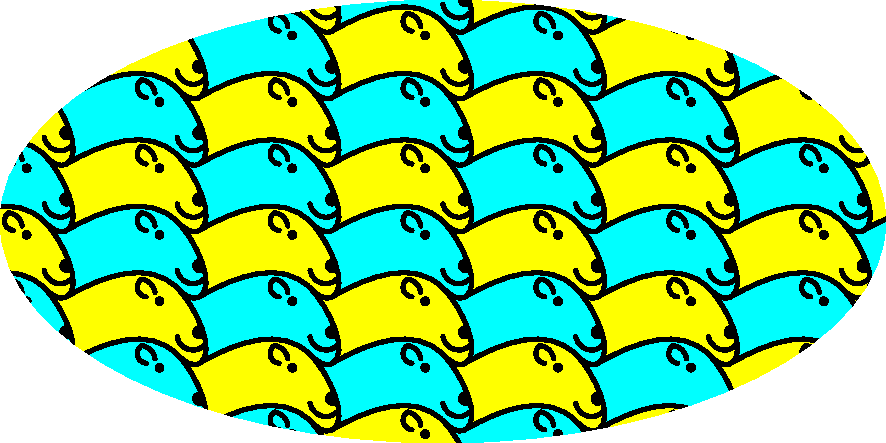
\includegraphics{tiling.pdf}
  \caption{André 理想中的铺砌图}
  \label{fig:tiling}
\end{figure}

André 很清楚他要画的图形的数学理论,但 André 的朋友 Timothy 告诉他要画这样
的图形多少是需要一些编程的知识的,对于他这样一位往日对计算机并不通晓的人来说
可能会有困难。不过 André 并不以为意:这世上还有什么比数学更难的呢?于是他兴
致勃勃的开始了。

\section{从矩形到铺砌}
\label{sec:rect2tiling}

铺砌图,顾名思义,就是像铺地板砖一样,把许多相同样式的图形平铺开来。不过,并
不是什么图形都可以平铺填满整个平面的——比如圆形就不行。把许多圆形一个挨一个
排列起来,也只能得到
\begin{figure}[H]
\centering
\begin{asy}
size(0,2cm);
for (int i = 0; i < 3; ++i)
    for (int j = 0; j < 10; ++j)
        filldraw(circle((j,i), 0.5), lightblue);
\end{asy}
\end{figure}
\noindent 或者是
\begin{figure}[H]
\centering
\begin{asy}
size(0,2cm);
for (int i = 0; i < 3; ++i)
    for (int j = 0; j < 10; ++j)
        filldraw(circle((j+0.5(i%2),sqrt(3)/2*i), 0.5), lightblue);
\end{asy}
\end{figure}
\noindent 都会留下许多空隙。而矩形、平行四边形、六边形等等都可以不留空隙地把平面铺满。

但问题是,如何设计出 André 理想中的那种看起来形状不规则的铺砌图案呢?

身为数学教师的 André 当然有办法。其实不规则铺砌图案还是规则图案的变形。
André 要画的羊形铺砌图,其实就是从矩形铺砌变化而来的。只要把一个矩形图案的上
下两边、左右两边分别变形,使得变形后的上边与下边、左边与右边还对应重合,就依
然可以完美地拼合起来。这正是铺砌图案最基本的构成方式:
\begin{figure}[H]
\centering
\begin{asy}
size(0,5cm);
defaultpen(linewidth(1mm));
path rec = box((0,0), (2,1));
draw(rec);

draw(shift(3,0)*rec, gray+0.5mm);
guide left = (0,1) -- (-0.2,0.8) -- (0,0.6) -- (0.1,0.1) -- (0,0);
guide bot = (0,0) -- (0.2,0.1) -- (1.6,-0.1) -- (2,0);
draw(shift(3,0) * (left ^^ shift(2,0)*left), heavyblue);
draw(shift(3,0) * (bot ^^ shift(0,1)*bot), heavygreen);

guide shape = left & bot & shift(2,0)*reverse(left)
    & shift(0,1)*reverse(bot) & cycle;
for (int i = 0 ; i < 2; ++i)
    for (int j = 0; j < 4; ++j)
	filldraw(shift(0.5+j,-1.5+0.5i)*scale(0.5)*shape, lightblue);
\end{asy}
\end{figure}

有了这个方法,对复杂的铺砌图,也只要从一个基本形状(比如矩形、正六边形)开始
变形,就等到铺砌所需要的一块“砖”。

因此,要画出羊头形状铺砌图,只要把一个矩形按照上面的要求变形为一个羊头形状,
在不同的位置重复画出就可以了。

\section{变量与曲线}

下面的问题就是,怎么画一个羊头呢?更具体地说,怎么画出羊头的曲线呢?

那么,首先要了解如何在 \Asy{} 中描述曲线。\ref{sec:linedraw} 节中提到 |--| 连
结一组坐标就成为直(折)线段;类似地,用 |..| 连结坐标就得到经过这些坐标点的
曲线:
\begin{lstlisting}
size(5cm,0);
pair z1 = (0,1), z2 = (1,1), z3 = (2,1),
     z4 = (0,0), z5 = (1,0), z6 = (2,0);
path p = z4 .. z1 .. z2 .. z6;
draw(p, gray+2mm);
\end{lstlisting}
\begin{figure}[H]
  \centering
\begin{asy}
size(5cm,0);
pair z1 = (0,1), z2 = (1,1), z3 = (2,1),
     z4 = (0,0), z5 = (1,0), z6 = (2,0);
path p = z4 .. z1 .. z2 .. z6;
draw(p, gray+2mm);
dot(Label("1", align=NW), z1);
dot(Label("2", align=NE), z2);
dot("3", z3);
dot("4", z4);
dot("5", z5);
dot("6", z6);
\end{asy}
\end{figure}

在这里,我们定义了一些变量\index{变量}以使代码清晰(这里略去了画点和标签的代
码)。|pair|\index{pair@\lstinline=pair=} 类型的变量 |z1|, \ldots, |z6| 保存
六个坐标\index{坐标},|path|\index{path@\lstinline=path=} 类型的变量 |p| 保存
一条曲线路径\index{路径}。因而上面 |size| 之后的绘图代码就相当于
\begin{lstlisting}
draw( (0,0) .. (0,1) .. (1,1) .. (2,0), gray+2mm );
\end{lstlisting}
其中前面的一句 |size(5cm,0)|\index{size@\lstinline=size=} 表示代码中的坐标只
是相对位置,最后将整个图形按比例放缩为 $5$\,cm 宽\footnote{注意坐标、图形会被
放缩,但画笔的宽度不会放缩。}。类似地,也可以使用 |size(0,4cm)| 把图形放缩到
$4$\,cm 高。

最重要的当然还是曲线的表示。以 |..| 连结的坐标会以一种尽量接近圆弧的方式连为
经过这些点的光滑曲线。与画直线类似,|cycle|\index{cycle@\lstinline=cycle=} 可
以作为一个特殊的坐标产生闭合曲线,即一条闭路径\index{路径!闭路径}:
\begin{lstlisting}
path q = z4 .. z1 .. z2 .. z6 .. cycle;
draw(q, gray+2mm);
\end{lstlisting}
\begin{figure}[H]
  \centering
\begin{asy}
size(5cm,0);
pair z1 = (0,1), z2 = (1,1), z3 = (2,1),
     z4 = (0,0), z5 = (1,0), z6 = (2,0);
path q = z4 .. z1 .. z2 .. z6 .. cycle;
draw(q, gray+2mm);
dot(Label("1", align=NW), z1);
dot(Label("2", align=NE), z2);
dot("3", z3);
dot("4", z4);
dot("5", z5);
dot("6", z6);
\end{asy}
\end{figure}

变量不仅仅是给了坐标、路径等对象一个简洁的名字,它也使得对同一个对象重复使用
并进行不同的操作变得十分方便:
\begin{lstlisting}
fill(q, lightblue);
draw(q, gray+2mm);
\end{lstlisting}
\begin{figure}[H]
  \centering
\begin{asy}
size(5cm,0);
pair z1 = (0,1), z2 = (1,1), z3 = (2,1),
     z4 = (0,0), z5 = (1,0), z6 = (2,0);
path q = z4 .. z1 .. z2 .. z6 .. cycle;
fill(q, lightblue);
draw(q, gray+2mm);
dot(Label("1", align=NW), z1);
dot(Label("2", align=NE), z2);
dot("3", z3);
dot("4", z4);
dot("5", z5);
dot("6", z6);
\end{asy}
\end{figure}

就像使用 |box| 可以直接得到矩形一样,最常用的曲线:圆、椭圆和圆弧,也可以使用
现成的命令得到:
\begin{table}[H]
\noindent
\begin{tabular}{ll}
|circle(c, r)| & 圆心 |c|,半径 |r| 的圆,这是逆时针方向的闭曲线; \\
|ellipse(c, a, b)| & 中心为 |c|,长半轴 |a|,短半轴 |b| 的椭圆,这也是逆时针
方向的闭曲线; \\
|arc(c, r, angle1, angle2)| & 圆心 |c|,半径 |r|,角度从 |angle1| 到 |angle2|
的圆弧。
\end{tabular}
\end{table}

例如:
\begin{lstlisting}
filldraw( circle((0,0), 1cm), lightblue, gray+2mm );
draw( arc((5cm,0), 1cm, 45, 135), gray+2mm );
\end{lstlisting}
\begin{figure}[H]
\centering
\begin{asy}
filldraw( circle((0,0), 1cm), lightblue, gray+2mm );
draw( arc((5cm,0), 1cm, 45, 135), gray+2mm );
\end{asy}
\end{figure}

一条用 |cycle| 产生的闭路径和简单地把首尾结点重合的路径是非常不同的。首先,只
有闭路径可以填充颜色;其次,使用 |cycle| 连结的曲线在起点处是光滑连接的,而如
果只是首尾结点重合则不会光滑连接。试将下面的曲线 |q2| 与上面的曲线 |q| 比较:
\begin{lstlisting}
path q2 = z4 .. z1 .. z2 .. z6 .. z4;
draw(q2, gray+2mm);
\end{lstlisting}
\begin{figure}[H]
\centering
\begin{asy}
size(5cm,0);
pair z1 = (0,1), z2 = (1,1), z3 = (2,1),
     z4 = (0,0), z5 = (1,0), z6 = (2,0);
path q2 = z4 .. z1 .. z2 .. z6 .. z4;
draw(q2, gray+2mm);
dot(Label("1", align=NW), z1);
dot(Label("2", align=NE), z2);
dot("3", z3);
dot("4", z4);
dot("5", z5);
dot("6", z6);
\end{asy}
\end{figure}

现在有了绘制曲线的方法,画出一个羊头就只是把草稿上的坐标连接起来而已。André
有一个纸上的草图,于是在描出几个点以后,他很快得到这样的结果(这里给图形增加
了辅助网格):
\begin{lstlisting}
size(0,4cm);
pen outline = black+1mm;
// `\color{comment}头`
path head = (0.5,-0.2) .. (0.6,0.5) .. (0.2,1.3) .. (0,1.5) .. (0,1.5)
    .. (0.4,1.3) .. (0.8,1.5) .. (2.2,1.9) .. (3,1.5) .. (3.2,1.3)
    .. (3.6,0.5) .. (3.4,-0.3) .. (3,0) .. (2.2,0.4) .. (0.5,-0.2) .. cycle;
filldraw(head, cyan, outline);
dot(head, red+1mm); // `\color{comment}画出羊头路径上的结点`
// `\color{comment}五官`
fill( circle((2.65,1.25), 0.12), outline );
fill( (3.5,0.3) .. (3.35,0.45) .. (3.5,0.6) .. (3.6,0.4) .. cycle, outline );
draw( (3,0.35) .. (3.3,0.1) .. (3.6,0.05), outline );
draw( (2.3,1.3) .. (2.1, 1.5) .. (2.15,1.7), outline );
draw( (2.1,1.7) .. (2.35,1.6) .. (2.45,1.4), outline );
\end{lstlisting}
\begin{figure}[H]
  \centering
\begin{asy}
size(0,4cm);
import math;
add(scale(1/2)*shift(0,-1)*grid(8,5,gray));
dot(Label("$O$",align=left), 0);
label("$1$", (0,1), align=W); label("$2$", (0,2), align=W);
label("$1$", (1,-0.5), align=S); label("$2$", (2,-0.5), align=S);
label("$3$", (3,-0.5), align=S); label("$4$", (4,-0.5), align=S);
pen outline = black+1mm;
path head = (0.5,-0.2) .. (0.6,0.5) .. (0.2,1.3) .. (0,1.5) .. (0,1.5)
    .. (0.4,1.3) .. (0.8,1.5) .. (2.2,1.9) .. (3,1.5) .. (3.2,1.3)
    .. (3.6,0.5) .. (3.4,-0.3) .. (3,0) .. (2.2,0.4) .. (0.5,-0.2) .. cycle;
filldraw(head, cyan, outline);
dot(head, red+1mm);
fill( circle((2.65,1.25), 0.12), outline );
fill( (3.5,0.3) .. (3.35,0.45) .. (3.5,0.6) .. (3.6,0.4) .. cycle, outline );
draw( (3,0.35) .. (3.3,0.1) .. (3.6,0.05), outline );
draw( (2.3,1.3) .. (2.1, 1.5) .. (2.15,1.7), outline );
draw( (2.1,1.7) .. (2.35,1.6) .. (2.45,1.4), outline );
\end{asy}
\end{figure}

在一开始,André 使用
\begin{lstlisting}
pen outline = black+1mm;
\end{lstlisting}
定义一个 |pen|\index{pen@\lstinline=pen=} 类型的变量 |outline| 表示用来画羊头
轮廓的画笔\index{画笔},以备使用。

然后,André 直接用 |..| 连结一组坐标来定义羊的头部轮廓:
\begin{lstlisting}
path head = (0.5,-0.2) .. (0.6,0.5) .. (0.2,1.3) .. (0,1.5) .. (0,1.5)
    .. (0.4,1.3) .. (0.8,1.5) .. (2.2,1.9) .. (3,1.5) .. (3.2,1.3)
    .. (3.6,0.5) .. (3.4,-0.3) .. (3,0) .. (2.2,0.4) .. (0.5,-0.2) .. cycle;
\end{lstlisting}
需要尖角的时候,就使用重复的相同点(如这里的起点);曲线变化大的地方,取的点
也比较密集。

最后五官的绘制。眼睛是填充的小黑圆,鼻子是黑色的卵形,耳朵和嘴都是简单的曲线。

于是,只要把这样一个图形一个挨一个地重复画许多遍,就可以得到 André 想要的铺
砌效果了。设计羊头形状的工作无疑是最关键也最复杂的,因此 André 的任务现在就
已经完成了一半。

不过继承了法国完美主义风气的 André 老师,很快挑出了毛病:这只羊头部的轮廓,
并不完全是按照 \ref{sec:rect2tiling} 节对矩形变形得到的——他的手稿基本上是这
样设计的,但在使用 \Asy{} 上绘图时则只是在手稿上相当随意地取了一些结点连结得
到曲线,这个轮廓想必也并不能严丝合缝地一个个拼起来。还有一件很令他恼火的事情
则是:要画出羊头的轮廓,他要画的点太多了,一个尖角用两个结点表示,也太不符合
他的简洁美学了。因此,这个看上去相当不错的羊头一号,就被 André 老师无情地否
决掉了。他决定发扬数学教师严谨简洁的作风,再做出更完美的羊头二号来。

\section{细致的曲线调整与曲线操作}

\section{子图和循环}

\section{路径剪裁}

\endinput

% vim:tw=77:

